
% % !TEX TS-program = xelatex
% % !TEX encoding = UTF-8 Unicode

% Spring 2020 - Summer 2020 - Fall 2020
% Tristan Hill, May 07, 2020 - June 12, 2020 - July 08, 2020 - Sept. 23
% Module 7 - Time Varying Circuits
% Topic 1 - The Dynamics of Circuits

\documentclass[fleqn]{beamer} % for presentation (has nav buttons at bottom)

\usepackage{/home/thill/Documents/lectures/measurements_lectures/measurements_lectures}

%\newcommand{\MNUM}{5\hspace{2mm}} % Module number
\newcommand{\TNUM}{2\hspace{2mm}} % Topic number 
\newcommand{\moduletitle}{Time Varying Circuits}
\newcommand{\topictitle}{First Order Systems} 

\newcommand{\sectiontitleI}{General System Model}
\newcommand{\sectiontitleII}{Mechanical-Electrical Analogies}
\newcommand{\sectiontitleIII}{Example: RC Circuit}
\newcommand{\sectiontitleIV}{Example: Bulb Thermometer}

% custom box
\newsavebox{\mybox}

\title{Lecture Module - \moduletitle}

\date{Mechanical Engineering\vspc Tennessee Technological University}

\begin{document}
	
	\lstset{language=MATLAB,basicstyle=\ttfamily\small,showstringspaces=false}
	
	\frame{\titlepage \center\begin{framed}\Large \textbf{Topic \TNUM - \topictitle}\end{framed} \vspace{5mm}}

% Section 0: Outline
\frame{
\large \textbf{Topic \TNUM - \topictitle} \vspace{3mm}\\

\begin{itemize}

	\item \sectiontitleI    \vspc % Section I
	\item \sectiontitleII 	\vspc % Section II
	\item \sectiontitleIII 	\vspc %Section III
	\item \sectiontitleIV 	\vspc %Section IV

\end{itemize}

}

% Section I:
\section{\sectiontitleI}

% Section I - Frame I:
\frame{  \small
\frametitle{\sectiontitleI}

The behavior of a circuit is dependent on time, and many common circuits can be represented by a {\it linear ordinary differential equation} which can be written in the following standard form. 

\[ a_n\frac{d^nx}{dt^n}+a_{n-1}\frac{d^{n-1}x}{dt^{n-1}}+...+a_2\frac{d^2x}{dt^2}+a_1\frac{dx}{dt}+a_0x=f(t) \] 
\vspace{0mm}

}


% Section II:
\section{\sectiontitleII}

% Section II - Frame I:
\frame{
\frametitle{\sectiontitleII}

Many mechanical systems are also time dependent, or {\it dynamic} and a mechanical-electrical analog is often draw between the two.

\renewcommand{\arraystretch}{1.5}
\begin{tabular}{ccc}
\underline{Zero Order}&\underline{First Order}&\underline{Second Order}\\
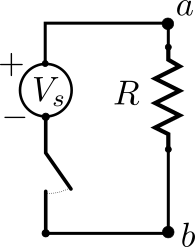
\includegraphics[scale=0.25]{r_circuit.png}&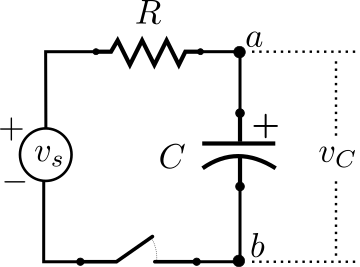
\includegraphics[scale=0.25]{rc_circuit.png}&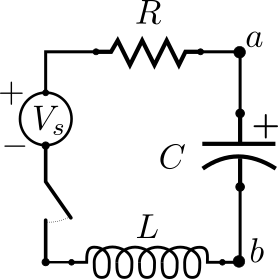
\includegraphics[scale=0.25]{rlc_circuit.png}\\
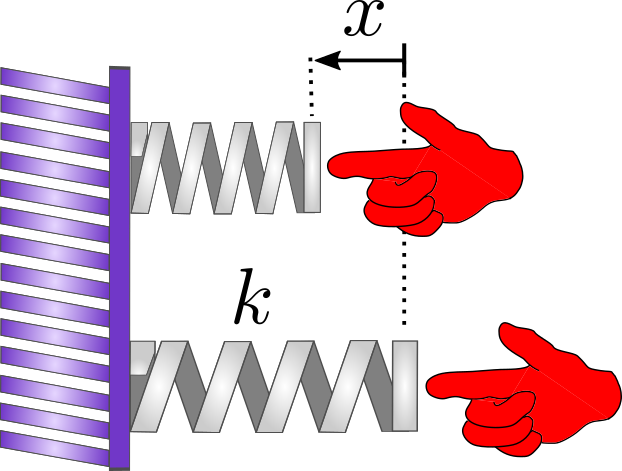
\includegraphics[scale=0.15]{hand_spring.png}&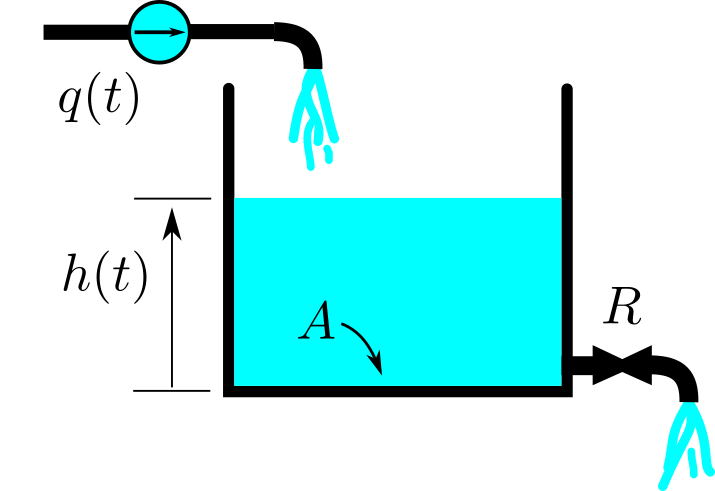
\includegraphics[scale=0.15]{water_tank.png}&\hspace{5mm}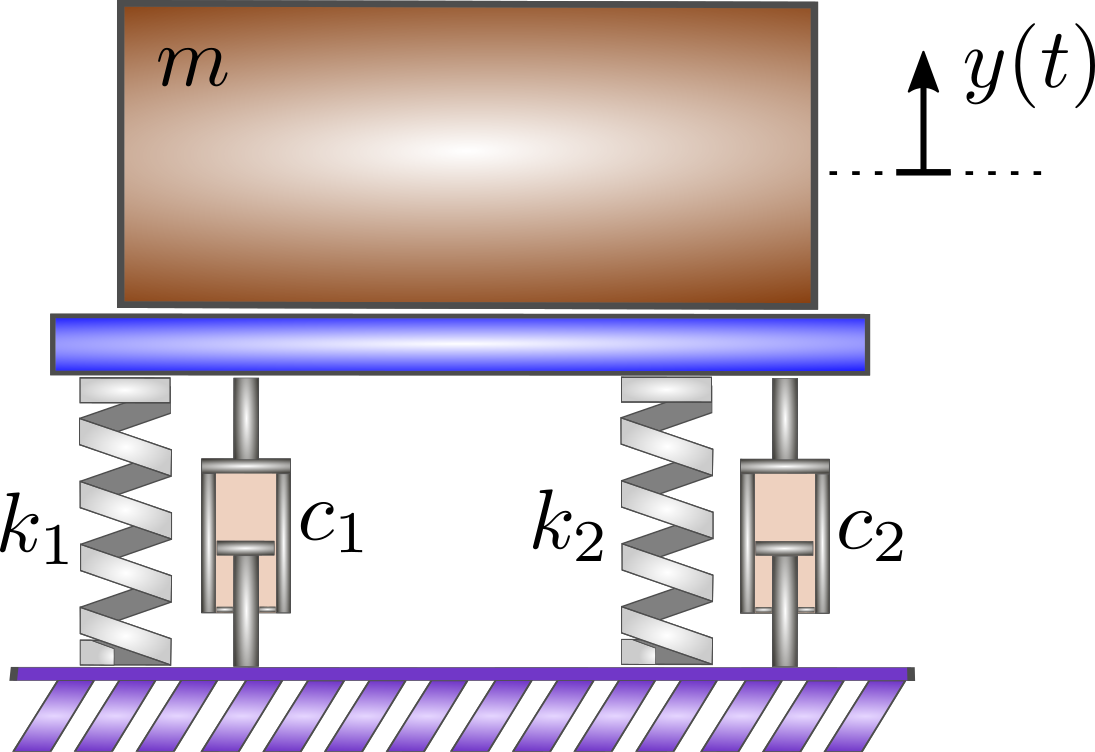
\includegraphics[scale=0.10]{mass_spring_damper.png}\\
\end{tabular}

This concept {\it was} used for analysis and simulation. 

}


% Section III:
\section{\sectiontitleIII}

% Section III - Frame I:
\frame{\small
\frametitle{\sectiontitleIII}

The RC circuit is a first order system. The response to a step input $v_s$ is exponential which is described a single parameter the time constant $\tau$. 
\vspc

\begin{multicols}{2}
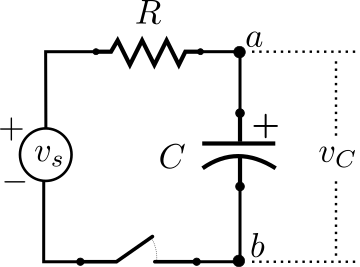
\includegraphics[scale=0.5]{rc_circuit.png} 	
	
First Order Model \vspace{15mm}\\
%\begin{fleqn}
%\[ RC\dot{v}_C+v_C=v_S \]
%\end{fleqn}

Response Equation
%\begin{fleqn}
%\[v_C\left(t\right)=v_s\left(1-e^{-\frac{t}{RC}}\right) \]
%\end{fleqn}

\end{multicols}


}

% Section III - Frame II:
\frame{\small
\frametitle{\sectiontitleIII}
	
\begin{multicols}{2}

\renewcommand{\arraystretch}{1.5}
\begin{tabular}{|c|c|} \hline
$time (s)$&$response (V)$\\ \hline
&\\ \hline
&\\ \hline
&\\ \hline
&\\ \hline
\end{tabular}

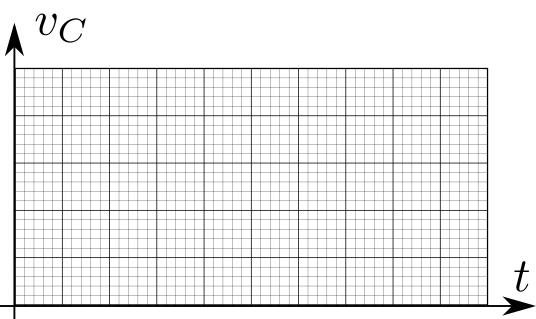
\includegraphics[scale=0.5]{voltage_versus_time.png} 	
\end{multicols}

	
}

%% Section IV:
\section{\sectiontitleIV}

% Section IV - Frame I:
\frame{ \small
\frametitle{\sectiontitleIV}

Consider the bulb thermometer shown which can be modeled as a first order system.  Where does the {\it model} come from? \vspc

\[ \frac{dE}{dt}=\dot{Q}\hspace{15mm} \frac{dE}{dt}=mc_v\frac{T(t)}{dt} \hspace{15mm}\dot{Q}=hA_s\Delta T \]
\[ \]

\begin{multicols}{2}

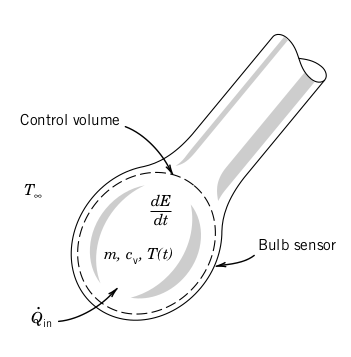
\includegraphics[scale=.35]{bulb_thermometer.png}

First Order Model \vspace{15mm}\\
%\begin{fleqn}
%\[ mc_v\frac{T(t)}{dt}+hA_sT(t)=hA_sT_\infty \] 
%\end{fleqn}

Response Equation
%\begin{fleqn}
%\[ T(t)=T_\infty+\left[ T\left(0\right)-T_\infty \right]e^{-\frac{t}{\tau}} \] 
%\end{fleqn}


\end{multicols}


}
	
% Section IV - Frame II:
\frame{ \small
\frametitle{\sectiontitleIV}

\begin{multicols}{2}

\renewcommand{\arraystretch}{1.5}
\begin{tabular}{|c|c|} \hline
$time (s)$&$response (^\circ C)$\\ \hline
&\\ \hline
&\\ \hline
&\\ \hline
&\\ \hline
\end{tabular}

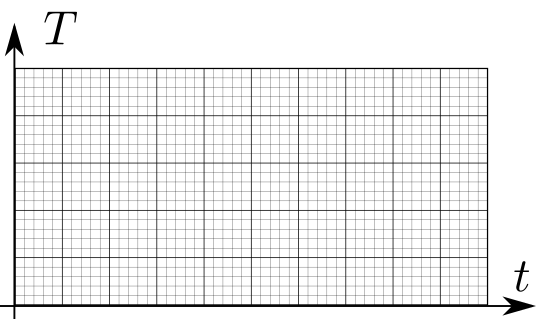
\includegraphics[scale=0.5]{temp_versus_time.png} 	
\end{multicols}


}
 
% Section IV - Frame III:
\frame{ \small
\frametitle{\sectiontitleIV}
Think about the {\it general system model}. \vspace{2mm}\\

What is the time constant of the bulb thermometer system? 

\vspace{5mm}
\begin{fleqn}
\[ \tau= \]
\end{fleqn}
\vspace{5mm}\\What is the static sensitivity? What are the units?
\vspace{5mm}
\begin{fleqn}
\[ K= \]
\end{fleqn}
\vspace{8mm}

}


\end{document}





